% COEN 6314 project - two-page data report, single-column article layout with a summary dashboard.
% Compile: pdflatex data_report_article.tex  (figures are read from fig/)
\documentclass[10pt,a4paper]{article}
\usepackage[a4paper,margin=1.7cm,top=1.5cm,bottom=1.6cm]{geometry}
\usepackage[T1]{fontenc}
\usepackage{lmodern}
\usepackage{microtype}
\usepackage{amsmath}
\usepackage{graphicx}
\usepackage{booktabs}
\usepackage{array}
\usepackage{xcolor}
\usepackage[most]{tcolorbox}
\usepackage{pgfplots}
\pgfplotsset{compat=1.18}
\usepackage{caption}
\usepackage{titlesec}
\usepackage{enumitem}
\usepackage[hidelinks]{hyperref}

\definecolor{ink}{HTML}{1F2933}
\definecolor{muted}{HTML}{616E7C}
\definecolor{accent}{HTML}{1D5C8C}
\definecolor{tile}{HTML}{EEF3F8}
\definecolor{ctrain}{HTML}{1D5C8C}
\definecolor{cval}{HTML}{E08A2E}
\definecolor{ctest}{HTML}{6B9F59}

\newcommand{\fn}[1]{\texttt{\detokenize{#1}}}
\titleformat{\section}{\normalfont\bfseries\color{accent}}{\thesection}{0.5em}{}
\titlespacing*{\section}{0pt}{6pt}{2pt}
\setlength{\parindent}{0pt}
\setlength{\parskip}{3pt}
\setlist{nosep,leftmargin=1.2em}
\captionsetup{font=footnotesize,labelfont=bf,skip=3pt}
\color{ink}

% dashboard tile: value, label
\newcommand{\kpi}[2]{%
  \begin{tcolorbox}[colback=tile,colframe=tile,arc=2pt,boxrule=0pt,left=1pt,right=1pt,top=2pt,bottom=2pt,
                    width=\linewidth,height=1.2cm,valign=center,halign=center]
  {\large\bfseries\color{accent}#1}\\[1pt]{\scriptsize\color{muted}#2}
  \end{tcolorbox}}

\begin{document}

%----------------------------------------------------------------- header
{\LARGE\bfseries PCB Defect Detection Under Image Misalignment}\\[2pt]
{\large Data Report}\hfill{\small Basma Kurany (40374114) \textperiodcentered{} COEN 6314, Concordia University
\textperiodcentered{} November 2026}\\[-4pt]
{\color{accent}\rule{\linewidth}{0.8pt}}

This report describes the data used to test whether a compact learned detector can separate genuine PCB defects
from misalignment artefacts: the DeepPCB source, the grouped partition, a quality audit of the raw pairs, the
seeded misalignment protocol, and the checks applied to every prepared image and box. All numbers come from the
scripts and JSON reports in the project repository.

%----------------------------------------------------------------- dashboard
\vspace{2pt}
\noindent
\begin{minipage}[t]{0.155\linewidth}\kpi{1,500}{image pairs}\end{minipage}\hfill
\begin{minipage}[t]{0.155\linewidth}\kpi{10,013}{defect boxes}\end{minipage}\hfill
\begin{minipage}[t]{0.155\linewidth}\kpi{\normalsize 800/200/500}{train / val / test}\end{minipage}\hfill
\begin{minipage}[t]{0.155\linewidth}\kpi{7,000}{val+test images}\end{minipage}\hfill
\begin{minipage}[t]{0.155\linewidth}\kpi{123}{natively misaligned}\end{minipage}\hfill
\begin{minipage}[t]{0.155\linewidth}\kpi{9/9}{checks passed}\end{minipage}

\vspace{4pt}
\noindent
\begin{minipage}[t]{0.60\linewidth}
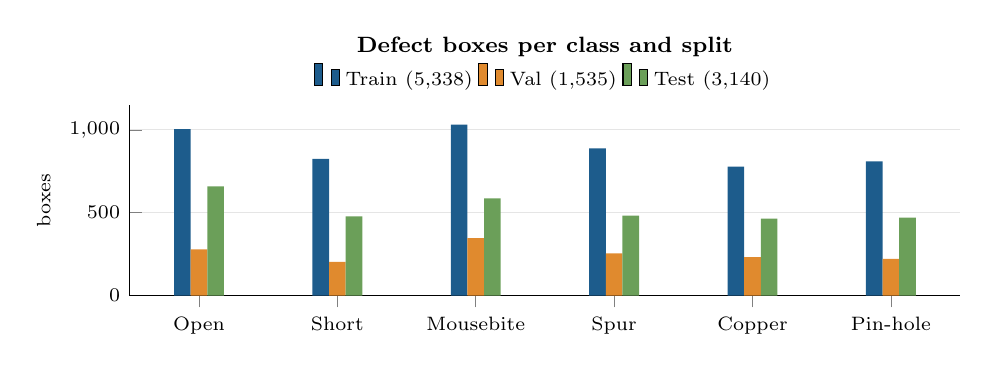
\begin{tikzpicture}
\begin{axis}[
  width=\linewidth, height=4.0cm, ybar=0pt, bar width=6pt,
  symbolic x coords={Open,Short,Mousebite,Spur,Copper,Pin-hole}, xtick=data,
  ymin=0, ymax=1150, ylabel={boxes}, ylabel style={font=\scriptsize},
  tick label style={font=\scriptsize}, axis lines*=left, ymajorgrids, grid style={gray!20},
  legend style={font=\scriptsize, draw=none, fill=none, at={(0.5,1.02)}, anchor=south, legend columns=3},
  title={\footnotesize\bfseries Defect boxes per class and split}, title style={yshift=8pt},
  enlarge x limits=0.1]
\addplot[fill=ctrain,draw=none] coordinates {(Open,1005) (Short,825) (Mousebite,1032) (Spur,888) (Copper,778) (Pin-hole,810)};
\addplot[fill=cval,draw=none]   coordinates {(Open,278) (Short,203) (Mousebite,347) (Spur,254) (Copper,232) (Pin-hole,221)};
\addplot[fill=ctest,draw=none]  coordinates {(Open,659) (Short,478) (Mousebite,586) (Spur,483) (Copper,464) (Pin-hole,470)};
\legend{{Train (5,338)},{Val (1,535)},{Test (3,140)}}
\end{axis}
\end{tikzpicture}
\end{minipage}\hfill
\begin{minipage}[t]{0.38\linewidth}
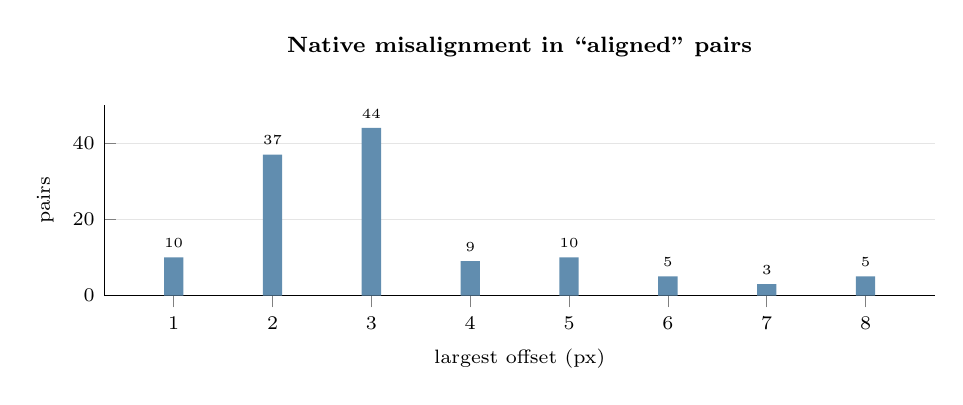
\begin{tikzpicture}
\begin{axis}[
  width=\linewidth, height=4.0cm, ybar, bar width=7pt, xtick={1,...,8},
  ymin=0, ymax=50, xlabel={largest offset (px)}, ylabel={pairs},
  label style={font=\scriptsize}, tick label style={font=\scriptsize},
  axis lines*=left, ymajorgrids, grid style={gray!20},
  nodes near coords, nodes near coords style={font=\tiny},
  title={\footnotesize\bfseries Native misalignment in ``aligned'' pairs}, title style={yshift=8pt}]
\addplot[fill=accent!70,draw=none] coordinates {(1,10) (2,37) (3,44) (4,9) (5,10) (6,5) (7,3) (8,5)};
\end{axis}
\end{tikzpicture}
\end{minipage}

%----------------------------------------------------------------- body
\section{Source dataset}
DeepPCB~\cite{tang2019} contains 1,500 pairs of $640\times640$ near-binary images: a defect-free \emph{template}
(reference) and an \emph{inspected} image of the same PCB region, aligned by the authors with template matching.
Each pair has 1--15 boxes (mean 6.7) labelled as open, short, mousebite, spur, spurious copper or pin-hole.
Defects are small (median $35\times33$\,px, about 0.3\,\% of the image) and classes are close to balanced
(largest/smallest ratio 1.33). Most defects were added artificially by the dataset authors, which limits claims
about real production defects. The official lists hold 1,000 \emph{trainval} and 500 \emph{test} pairs from 11
source-board \emph{groups}; the group folder is the only board identifier available.

\section{Partition}
The official 1,000/500 split is kept. About 20\,\% of trainval is held out for validation \emph{before} any
augmentation, grouped by board so that no board appears in both train and validation. Every subset of trainval
groups with 17--23\,\% of the pairs was scored by the $L_1$ distance between its class proportions and those of
all trainval; the best is group \fn{00041} (200 pairs, $L_1=0.059$). All shifted variants of a pair inherit the
pair's split. Because the official test list was kept, the rule ``same board, same partition'' cannot hold for
test: 168 test pairs come from 7 groups also present in trainval (21 from the validation group). The other 332
come from four groups never seen in trainval (\fn{12000}, \fn{12100}, \fn{12300}, \fn{90100}), so a
group-held-out validation set is a reasonable proxy for test.

\section{Data-quality audit}
\begin{itemize}
\item \textbf{Format.} All 3,000 images are $640\times640$; 62 images in 57 pairs are 3-channel JPEGs and were
converted to single-channel PNG. No label file is empty, malformed or out of bounds.
\item \textbf{Near-duplicates.} A difference hash over all templates gave 337 candidates, re-checked at pixel
level (best offset within $\pm8$\,px, Jaccard $\geq0.9$). 40 duplicates were confirmed, all inside one group,
which supports group as the board unit. None crosses train/val; three test pairs (\fn{50600065},
\fn{92000114}, \fn{92000118}) duplicate a train pair and are flagged for a with/without comparison.
\item \textbf{Native misalignment.} An integer search ($\pm8$\,px) for the offset that minimises
template/inspected disagreement finds 123 pairs (8.2\,\%; 75 train, 8 val, 40 test) where an offset cuts the XOR
area by at least $1.5\times$, typically 2--3\,px (chart above, Fig.~\ref{fig:native}). Their ``aligned'' condition
is therefore already shifted. Offsets are stored per pair, so results can be reported on all pairs and, as a
sensitivity check, on the 1,377 clean pairs (460 in test). 17 templates are near-blank.
\end{itemize}

\begin{figure}[h]
\centering
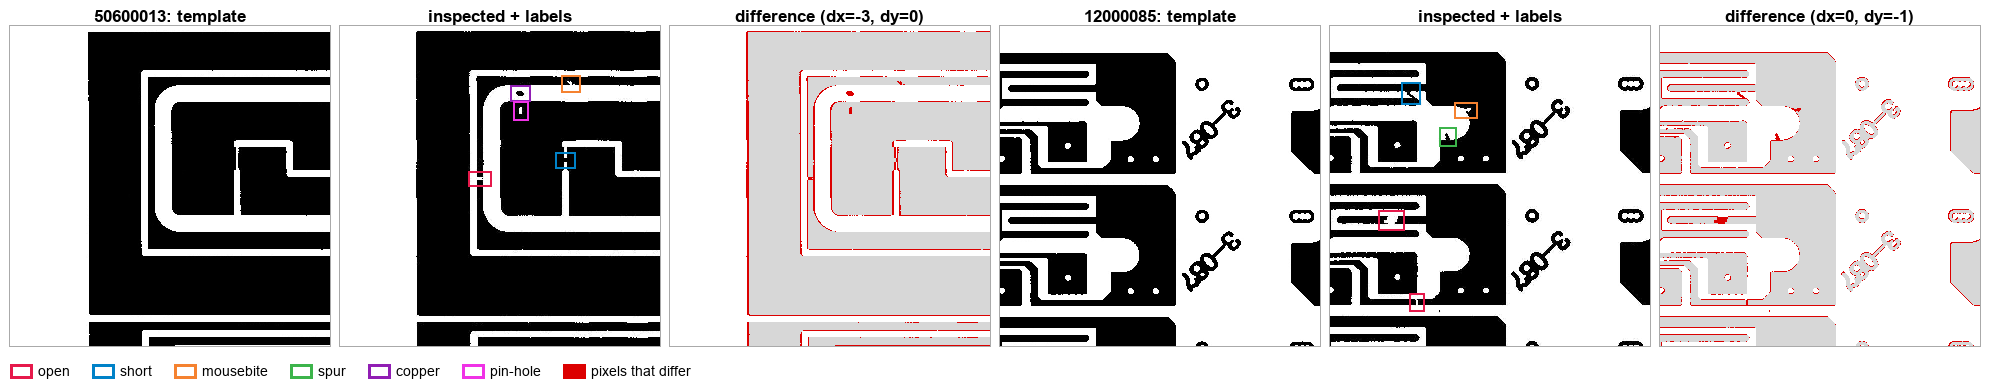
\includegraphics[width=0.9\linewidth]{fig/native_misalignment_white_row.png}
\caption{Two pairs supplied as ``aligned'' but offset by 3\,px and 1\,px (offset found by the audit). Boxes show
the labelled defects by class; red marks pixels that differ between template and inspected image.}
\label{fig:native}
\end{figure}

\section{Controlled misalignment protocol}
The reference is never modified; the inspected image and its boxes move together. Each validation and test pair
gets ten conditions (Table~\ref{tab:conds}): the pair as supplied (\fn{s0}); integer shifts of 1, 2, 3 and
5\,px along $x$ or $y$ with a random sign; and a \emph{residual} condition $r$ (sub-pixel translation of
0.25--1.5\,px plus a rotation within $\pm0.5^\circ$) that whole-pixel registration cannot undo exactly.
Integer shifts copy pixels, so they add no interpolation artefacts; $r$ uses bilinear interpolation, and rotated
boxes become the axis-aligned envelope of their corners. Parameters come from a generator seeded with
$(6314,\text{pair ID})$, so the baseline and the detector read the \emph{same} files. \textbf{Training
does see misalignment:} the non-augmented run uses the 800 pairs as supplied (75 already natively offset), and the
augmented run adds one random 1--5\,px shift and one residual copy of every pair (2,400 images, separate seed
stream; Section~6).

\begin{table}[h]
\centering\small
\begin{minipage}[t]{0.47\linewidth}\centering
\captionof{table}{Prepared inspected images.}\label{tab:conds}
\begin{tabular}{@{}lcccr@{}}
\toprule
Split & \fn{s0} & 1/2/3/5\,px $\times\{x,y\}$ & $r$ & Images\\
\midrule
Train & 800 & -- & -- & 800\\
Val   & 200 & $8\times200$ & 200 & 2,000\\
Test  & 500 & $8\times500$ & 500 & 5,000\\
\bottomrule
\end{tabular}
\end{minipage}\hfill
\begin{minipage}[t]{0.50\linewidth}\small
\textbf{Borders and truncated defects.} Uncovered pixels are edge-replicated inside an 8\,px border that
evaluation excludes. A box whose \emph{original} position is within 14\,px of an edge is marked \emph{ignore} in
every condition (258 boxes, 2.6\,\%): it counts as neither hit nor miss, and a prediction matching it is not a
false positive.
\end{minipage}
\end{table}

\section{Verification}
Two sets of checks were run: the pipeline's own QA scripts, and an independent audit that re-decodes the raw
DeepPCB files with a different library (Pillow/SciPy instead of OpenCV) and does not reuse the pipeline code.
The only difference found is one colour JPEG (\fn{44000020}) whose grey conversion differs between decoders on
2\,\% of pixels; its shifted copies still match its own \fn{s0} exactly.

\noindent
\begin{minipage}[t]{0.50\linewidth}\vspace{0pt}
\small
\begin{tabular}{@{}p{0.76\linewidth}r@{}}
\toprule
Check & Result\\
\midrule
Pair lists, splits, \fn{boxes.csv} match raw & 1500/1500\\
References identical to raw templates & 1500/1500\\
\fn{s0} identical to raw (independent decoder) & 1499/1500\\
Integer shift $=$ \fn{s0} moved by $(dx,dy)$ & 5600/5600\\
Box count, class, offset, ignore flag & 52088/52088\\
Non-ignored boxes in valid region & 41220/41220\\
Residual images reproduced from parameters & 700/700\\
COCO files consistent with CSV & 21/21\\
YOLO images with labels, zip CRC intact & 10200/10200\\
\bottomrule
\end{tabular}
\end{minipage}\hfill
\begin{minipage}[t]{0.47\linewidth}\vspace{0pt}
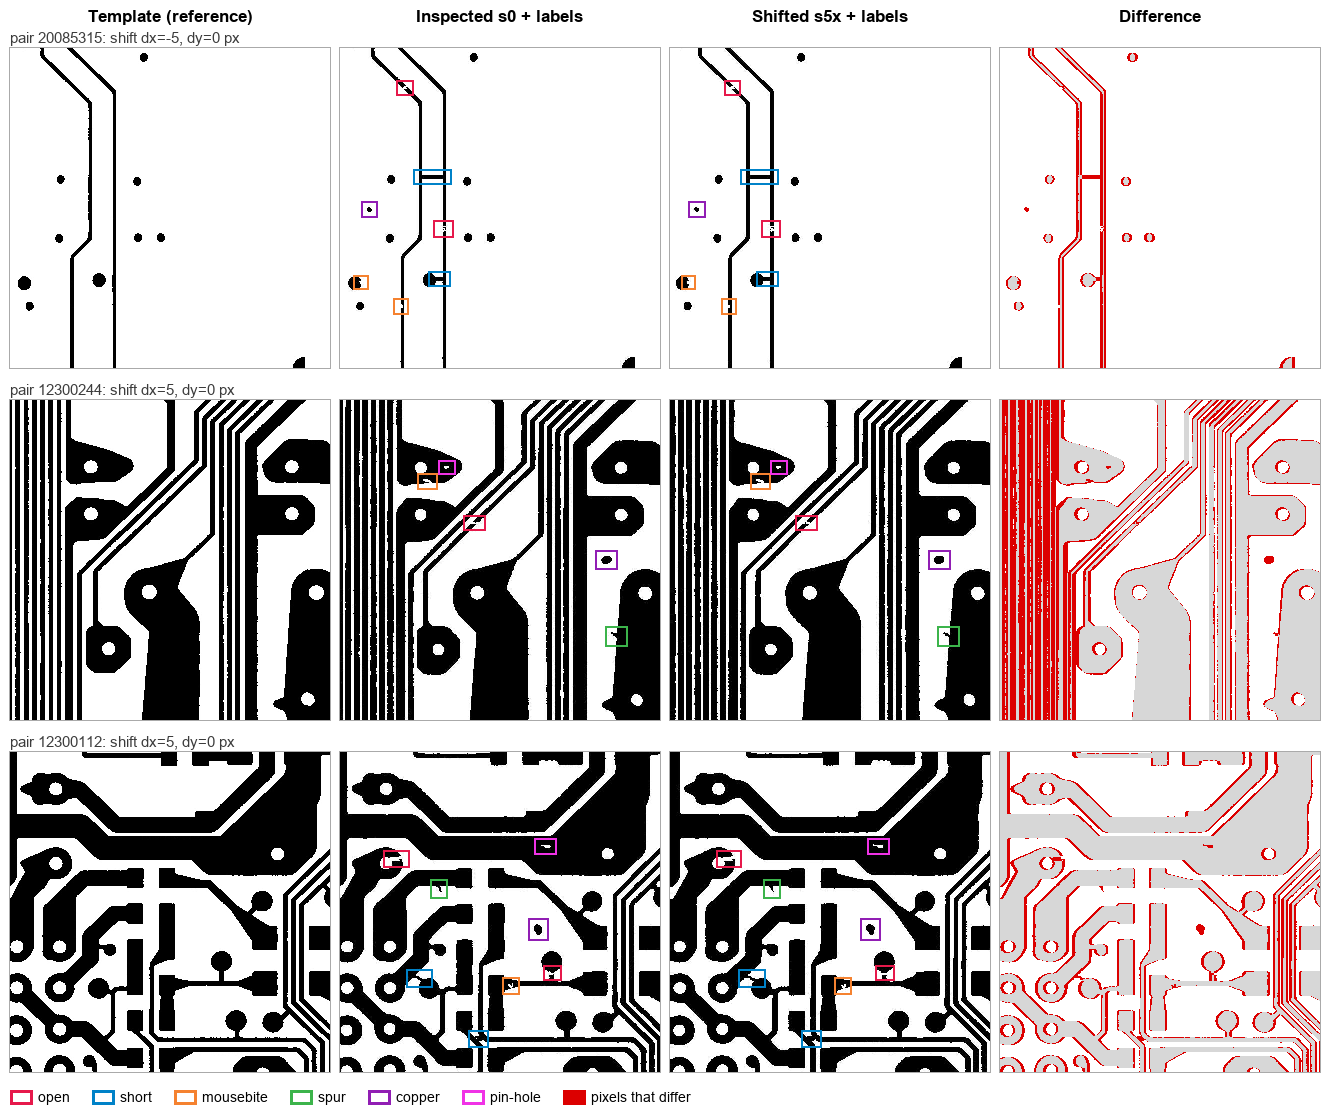
\includegraphics[width=\linewidth]{fig/check_s5x_white.png}
\captionof{figure}{Label check, 5\,px shift: template; inspected \fn{s0} with labels; shifted image with shifted
labels; difference in red, where every track edge becomes a false difference.}
\end{minipage}

\section{Model-ready formats and reproducibility}
The master format is CSV: \fn{splits.csv} (pair, group, split, native offset, duplicate flag), \fn{images.csv}
(one row per inspected image with $dx$, $dy$, rotation) and \fn{labels.csv} (one row per box with class and ignore
flag). The same data are exported as 21 COCO files and as a YOLO package where each pair is one 3-channel image
(reference, inspected, $|$difference$|$), so an RGB-pretrained YOLOv10-Nano takes both images unchanged. The
augmented run (3$\times$ the images) trains for one third of the epochs, so both runs take the same number of
steps. Colour augmentation stays off
because it would corrupt the difference channel; YOLO cannot encode ignore boxes, so evaluation reads
\fn{labels.csv}. Everything is rebuilt from the untouched DeepPCB download with \fn{scripts/run_all.sh}.

\section{Limitations}
Most defects are synthetic; validation is a single board group; each pair has one residual variant; 123 pairs are
natively misaligned; and 168 test pairs share a board with trainval. These are reported with every result rather
than corrected.

\vspace{-4pt}
\begin{thebibliography}{1}\footnotesize
\bibitem{tang2019} S.~Tang, F.~He, X.-L.~Huang, and J.~Yang, ``Online PCB defect detector on a new PCB defect
dataset,'' \emph{arXiv:1902.06197}, 2019.
\end{thebibliography}
\end{document}
